\chapter{Punktesortierung in Schachbrettmustern}
\label{sec:schachbrettAlg} 


Für die Detektion von korrespondierenden Punkten in Stereoskopischen Bildaufnahmen von zweidimensionalen Schachbrettern, ist ein Algorithmus entwickelt worden, welcher die zuvor Detektierten Eckpunkte eines Schachbretts sortiert und eindeutig identifiziert. Jeder Punkt beinhaltet nach der Sortierung die Information in welcher Reihe $j$ und in welcher Spalte $i$ er sich befindet. Jeder Punkt ist somit eindeutig durch die zwei Indizes $i$ und $j$ identifiziert. Dem entstandenen Sorierungsalgorithmus ist ein Algorithmus zu Detektion der Eckpunkte eines Schacbretts voran geschaltet. Werden beide Algorithmen auf die Stereoaufnahme zweier Schachbretter angewandt, so können korrespondierende Punkte anhand dieser Indizes ausgemacht werden. Die Schachbretter können dabei sowohl Kissen- als auch Tonnennverzeichnungen aufweisen und oder perspektivisch verzerrt sein.\\ 



%Das Bild des Schachbretts wird in ein zweidimensionales Koordinatensystem $(A,\alpha)$ mit $\alpha = (j,i)$ gelegt. 

%Als erstes wird ein Startpunkt innerhalb des Schachbretts gesucht. 

Aus den zuvor detektierten Eckpunkten des Schachbretts wird ein Startpunkt gesucht. Der Startpunkt wird so bestimmt, dass es immer die linke unterste Ecke des Schachbretts ist. Somit ist gewährleistet, dass die Indizes der Eckpunkte beider Bilder gleich sind. Ist der Startpunkt bestimmt, bekommt dieser die Indizes $i = 1$ und $j = 1$. $i$ steht für die jeweilige Reihen in welcher sich ein Punkt befindet und $j$ steht für die jeweilige Spalte. Ist der Startpunkt bestimmt, wird der erste Punkt entlang der unteren Schachbrettkante in $j$-Richtung und der erste Punkt entlang der linken Randkante in $i$-Richtung gesucht. Anhand dieser Punkte lassen sich vom Startpunkt aus Richtungsvektoren definieren. Entlang des Richtungsvektors wird ein Bereich definiert. In Abbildung \ref{fig:UebersichtSortierungsAlg} ist dieser Suchbereich als das blaue Dreieck dargestellt. Ist der nächste Punkt gefunden, so wird der Richtungsvektor anhand des zu vorigen und des neuen Punktes neu ausgerichtet. Der dynamische Suchbereich ermöglicht es somit, dass selbst bei stark verzerrten Schachbrettern, bei denen Punkte nicht mehr auf einer Gerade liegen, Punkte der einzelnen Reihen und Spalten des Schachbretts ausfindig gemacht werden können.


\begin{figure}[!htb]
	\centering
	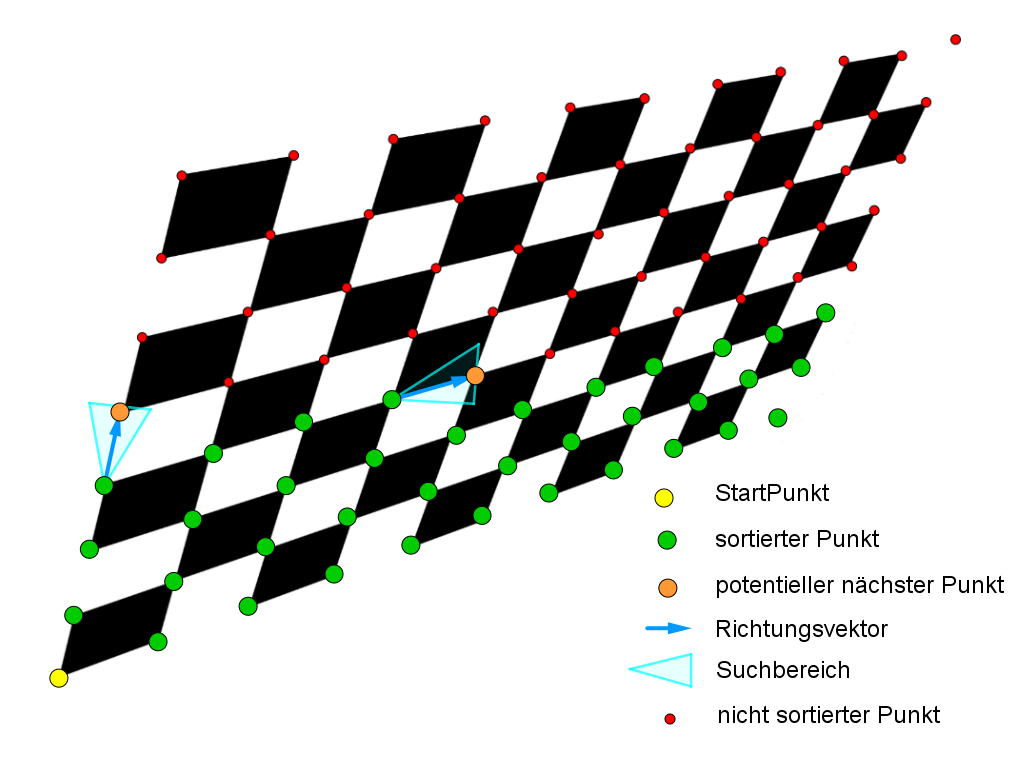
\includegraphics[width=0.8\linewidth]{images/VerzeichnetesSchachbretFunktion.png}
	\caption[Funktionsübersicht des Sorieralgorithmus]{In der Abbildung ist die Vorgehensweise des Sortierungsalgorithmus schematisch zu sehen.}
	\label{fig:UebersichtSortierungsAlg}
\end{figure}




\section{Sortierungsalgorithmus}

Im Folgenden soll der Ablauf des implementierten Sortierungsalgorithmus beschrieben werden und dessen Funktionsweise an Beipspielen von unterschiedlichen Schachbrettern demonstriert werden.\\

Der Soritierungsalgorithmus nimmt eine Liste aus den unsortierten Eckpunkten des Schachbretts entgegen. Von den Punkten in dieser Liste wird eine grobe Vorsortierung vorgenommen.

Um das Schachbrett herum wird ein Rahmen definiert. Die Punkte mit der maximalen $y$-Koordinate und der minimalen $y$-Koordinate Begrenzen die oberen und unteren Kanten des Rahmens. Die Punkte mit der minimalen $x$-Koordinate und der Punkt mit der  maximalen $x$-Koordinate begrenzen die vertikalen Kanten des Rahmens. In Abbildung \ref{fig:7.1} sind die roten Begrenzungskanten um das Schachbrett zu sehen.\\

\begin{figure}[!htb]
	\centering
	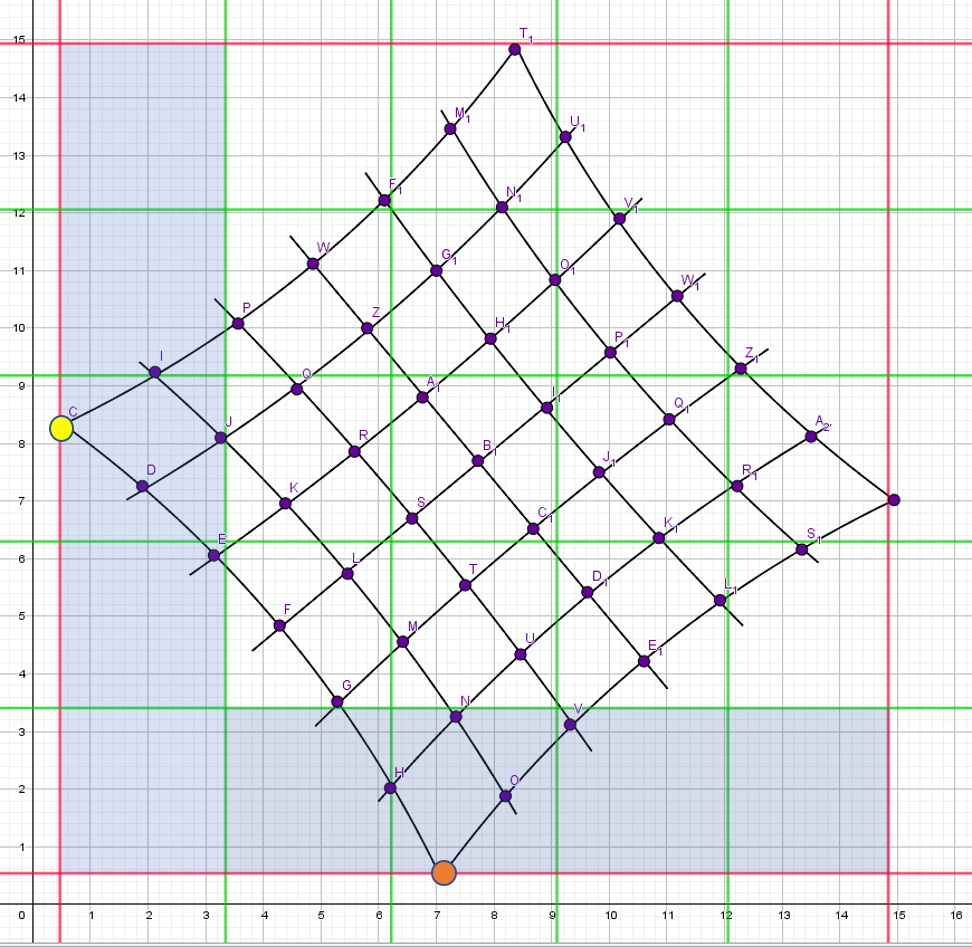
\includegraphics[width=0.6\linewidth]{images/VerzeichnetesSchachbrett_1.png}
	\caption[Startpunktsuche in Schachbrettpunkten]{Die in blau markierten Bereiche beinhalten die möglichen Startpunkte. Der Bereich entlang der horizontalen $j$- Achse bildet die erste Suchfensterreihe in $i$-Richtung. Der blaue Bereich entlang der vertikalen $i$-Achse bildet die erste Suchfensterreihe in $j$-Richtung. Der gelbe Punkt steht für den Punkt welcher als $VecJ$ bezeichnet wurde und der orange Punkt ist derjenige Punkt, welcher als $VecI$ bestimmt wurde}
	\label{fig:7.1}
\end{figure}

Der durch den Rahmen begrenzte Bereich, welcher das gesamte Schachbrett einschließt, wird in mehrere Zellen eingeteilt. Diese werden durchgezählt und mit den Indizes $i$ und $j$ eindeutig bestimmt. $i$ beschreibt die Reihennummer der Zelle und $j$ beschreibt die entsprechende Spalte. In Abbildung \ref{fig:7.1} hätte die Zelle links unten im Eck somit die Indizes $i = 1$ und $j = 1$, die zweite rechts daneben die Indizes $i = 1$ und $j= 2$.\\

In zwei $ConstantArrays$ namens $JSplits$ und $ISplits$ werden die Begrenzungen de Zellen  in $x$- und $y$-Richtung gespeichert. Die Begrenzungen der Zellen werden berechnet, idem die  Distanz zischen den vertikalen und horizontalen Kanten des Rahmens durch die gewünschte Anzahl an Zellen geteilt wird.\\  

Im nächsten Schritt wird überprüft welche Punkte innerhalb welcher Zellen liegen. Für jeden Punkt wird eine Liste Aus $Associations$ angelegt.  $Associations$ können Werten Schlüsselwörter zuweisen. Anhand dieser Schlüssel sind Werte eindeutig identifiziert\cite{Mathematica}. Pro Punkt werden die jeweils die $x$- und $y$-Koordinaten und die Indizes Zellen in Schlüssel gespeichert.

\begin{gather*}
	Punkt = \, \{<|Coordx \rightarrow x_u, Coordy \rightarrow y_u, CellI \rightarrow i_u, CellJ \rightarrow j_u |>\}
\end{gather*} \\

In Abbildung \ref{fig:7.1} sind die Zellen durch die grünen Linien begrenzt. Die Vorsortierung in Zellen macht es im weiteren Verlauf der Sortierung der Punkte in Zeilen un Spalten einfacher, wenn es darum geht nur bestimmte Bereiche des Schachbretts zu untersuchen.\\

Nach der Vorsortierung wird der Punkt gesucht, von welchen aus das Schachbrettgitter rekonstruiert werden soll. Alle Punkte innerhalb den Zellen mit den Indizes $i=1$ und $j \leq  j_{max}$ und $i \leq i_{all}$ und $j = 1$ werden als mögliche Startpunkte gekennzeichnet. In Abbildung \ref{fig:7.1} befinden sich die möglichen Startpunkte innerhalb des blau hinterlegten Bereichs.\\

%Die Suche nach einem Startpunkt und auch nach den ersten Punkten in zwei Richtungen vom Startpunkt aus, ist relativ komplex. Der Grund hierfür ist, dass sämtliche Schachbretter wie in \ref{sec:SchachAlgBeispiele} gezeigt, in Betracht gezogen werden müssen. 

Um Anhand des Algorithmus später korrespondierende Punkte in zwei Aufnahmen des Schachbretts finden kann, sollte gewährleistet sein, dass der Startpunkt immer an der selben Ecke eines Schachbretts platziert wird.\\

%Innerhalb der blau gefärbten Fläche, wie sie in Abbildung \ref{fig:7.1} abgebildet ist, wird nach einem Startpunkt gesucht. 
%
%
%Die Suche nach einem Startpunkt wird pro $i$- und $j$-Richtung in zwei Abfragen unterteilt.\\
Die jeweiligen horizontalen Zellen $i=1$ und $j \leq  j_{max}$ werden getrennt von den vertikalen $i \leq i_{all}$ und $j = 1$ untersucht. Innerhalb der horizontalen Zellen wird zunächst nach dem Punkt mit der kleinsten $y$-Koordinate gesucht und als erster möglicher Startpunkt in $VecI$ gespeichert. Danach wird überprüft, ob es einen Punkt gibt, dessen $x$-Koordinate kleiner ist als die des momentan gesetzten $VecI$. Ist dies der Fall so wird noch überprüft, ob dessen $y$-Koordinate kleiner gleich der von $VecI$ plus einem Pufferwert ist. Der Pufferwert wird so definiert, dass die $y$-Koordinate des neuen möglichen $VecI$ zwar größer als die des momentanen sein kann, jedoch eine bestimmte Schwelle nicht übertreten darf, da es sich sonst um einen Punkt der zweiten $i$-Reihe handeln könnte. In Abbildung \ref{fig:7.1} ist $VecI$ als oranger Punkt abgebildet.\\

Innerhalb des vertikalen Suchbereichs bestehend aus den Zellen  $i \leq i_{all}$ und $j = 1$ wird derjenige Punkt gesucht, dessen $x$-Koordinate minimal ist und wird als Punkt $VecJ$ gespeichert. Im nächsten Schritt wird ein Punkt innerhalb des Bereichs gesucht, dessen $y$-Koordinate kleiner ist als die des momentanen $VecJ$ und dessen $x$-Koordinaten kleiner gleich der $x$-Koordinate von $VecJ$ plus einem Pufferwert ist. Ist so ein Punkt gefunden, wird dieser als neues $VecJ$ bestimmt. $VecJ$ ist in Abbildung \ref{fig:7.1} als gelber Punkt dargestellt.\\

%Für die erste Abfrage in $j$-Richtung, werden die Zellen entlang der vertikalen $i$-Koordinatenachse mit den Indizes $j=1$ und $i \leq i_{max}$, nach dem Punkt gesucht, welcher die geringste $j$-Koordinate besitzt. Dieser Punkt wird als vorläufiges $VecJ$ bestimmt.\\
%
%Danach wird auch hier geprüft, ob es innerhalb der ersten Suchfensterreihe in $j$-Richtung einen weiteren Punkt gibt, dessen $i$-Koordinate kleiner ist als die des momentan gesetzten Punktes $VecJ$. Trifft des Weiteren zu, dass die $j$-Koordinaten des neu gefundenen Punktes kleiner ist als die $j$-Koordinate plus einem Pufferwert des momentanen $VecJ$ , so wird dieser als neuer Punkt als $VecJ$ festgelegt. In Abbildung \ref{fig:7.1} ist $VecJ$ als gelber Punkt zu sehen.\\

Je nachdem wie das Schachbrett rotiert ist oder welche Art der Verzerrungen es aufweist, kann es sein dass $VecI$ und $VecJ$ bereits den selben Punkt ergeben haben, was den Startpunkt $StartPoint$ eindeutig identifiziert, wie es in den  Beispielen \ref{fig:Extreme1} oder auch \ref{fig:Extreme5} der Fall ist. Andererseits kann es auch wie in Abbildung \ref{fig:7.1} zu sehen ist, sein, dass $VecI$ und $VecJ$ sich unterscheiden. In solchen Fällen wird $VecJ$ als Startpunkt festgelegt. Damit ist gewährleistet, dass je nach Lage des Schachbretts der linke obere oder die linke untere Ecke des Schachbretts als Startpunkt gesetzt werden\\

Die $Assiciation$-Liste des Startpunktes wird um zwei weitere Schlüssel erweitert. Die Schlüssel $NeighbourI$ und $NeighbourJ$ speichern die Werte in welcher Reihe $i$ und welcher Spalte $j$ des Schachbrettgitters sich der gefundenen Punkt befindet. Der Startpunkt $StartPoint$ ist dann wie folgt definiert


% $Associations$ können Werten Schlüsselwörter zuweisen. Anhand dieser Schlüssel sind Werte eindeutig identifiziert. 

%Die $Association$-Liste $SortedPoints$ beinhaltet die Schlüssel $CoordJ$ und $CoordI$, welche die jeweiligen $i$- und $j$- Koordinaten des Punktes speichern. Die Schlüssel $CellI$ und $CellJ$, speichern 
%
%die Information in welcher Zelle sich der Startpunkt befindet und die Schlüssel $NeighbourI$ und $NeighbourJ$ speichern die Indizes $i$ und $j$ ab, die definieren, der wievielte Punkt $StartPoint$ in $i$-Richtung und in $j$-Richtung ist. Er bekommt als erster Sortierter Punkte die $NeighbourI = 1$ und $NeighbourJ = 1$ zugeordnet. Ein Eintrag für einen Punkt in der Liste $SortedPoints$ sieht wie folgt aus \\

\begin{gather*}
	\begin{split}
			StartPoint &= \{ <|Coordx \rightarrow x-_u,\, Coordy \rightarrow y_u,\, \\
			&CellI \rightarrow i_u,\, CellJ \rightarrow j_u,\,
			NeighbourI \rightarrow 1, \,NeighbourJ \rightarrow 1 |>\}
	\end{split}
\end{gather*}
 
Anhand der Schlüssel $NeighbourI$ und $NeighbourJ$, ist die Position des Punktes innerhalb des Schachbrettgitters eindeutig identifiziert. Somit können in einer Stereoskopischen Aufnahme die korresponierenden Eckpunkte von Schachbrettern identifiziert werden. In Abbildung \ref{fig:ChessBoardLeftAlg} und \ref{fig:ChessBoardRightAlg} wurde in beiden Bildern alle Punkte abgefragt, deren Schlüssel $NeighbourI = 3$ ist. Die grün gefärbten Punkte liefern das Ergebnis. \\

$StartPoint$ wird danach in zwei unterschiedliche Listen geschrieben. Die Liste $SortedPoints$ speichert alle fertig sortierten Punkte. Die Liste $CheckList$ speichert eine verkürzte $Associtaion$- Liste der Punkte, welche nur aus den Schlüsseln $Coordx$ und $Coordy$ besteht. Anhand der in $Checklist$ gespeicherten Koordinaten eines Punktes, soll bei der weiteren Suche verhindert werden, dass ein Punkt mehrmals als sortiert wird.\\



%In den Abbildungen \ref{fig:Extreme1} bis \ref{fig:Extreme10} wurden die Punkte angefragt welche sich in der dritten Reihe von $i$ befinden. Besagte Punkte sind in den Grafiken grün eingefärbt.\\
%
%Die Schlüssel $ICoord$ und $JCoord$ werden noch in eine weitere Liste namens $CheckList$ gespeichert. Anhand der $CheckList$ wird überprüft, ob die Koordinatend und somit ein Punkt selbst bereits Sortiert wurde. Damit wird verhindert, dass ein Punkt mehrmals in einsortiert wird.\\
% 
Nachdem der Startpunkt gefunden ist werden die jeweils nächsten Punkte in $i$- und $j$-Richtung gesucht. Diese Punkte werden dann in die Variablen $NextI$ und $NextJ$ gespeichert. In Abbildung \ref{fig:NextINextJ} ist $NextI$ der violette Punkte und $NextJ$ ist der rote Punkte. \\

Für die Bestimmung von $NextI$ wird zu erst initial $NextI = <|Coordx \rightarrow 100 000, Coordy \rightarrow 100 000|>$ gesetzt. Für den Punkt $NextI$ der nächsten Reihe $i$ wird die Zelle in welchem sich $StartPoint$ befindet und die jeweiligen Zellen eins darüber und darunter durchsucht. In Abbildung \ref{fig:NextINextJ} ist dieser Bereich um $StartPoint$ gelb hinterlegt. 

%Es werden Punkte gesucht, welche sich in der selben $CellI$ wie $StartPoint$ und in den Zellen eins darüber $CellI +1$ und eine darunter $CellI-1$ befinden. In Abbildung \ref{fig:NextINextJ} ist der Bereich gelb eingefärbt.\\


\begin{figure}[!htb]
	\centering
	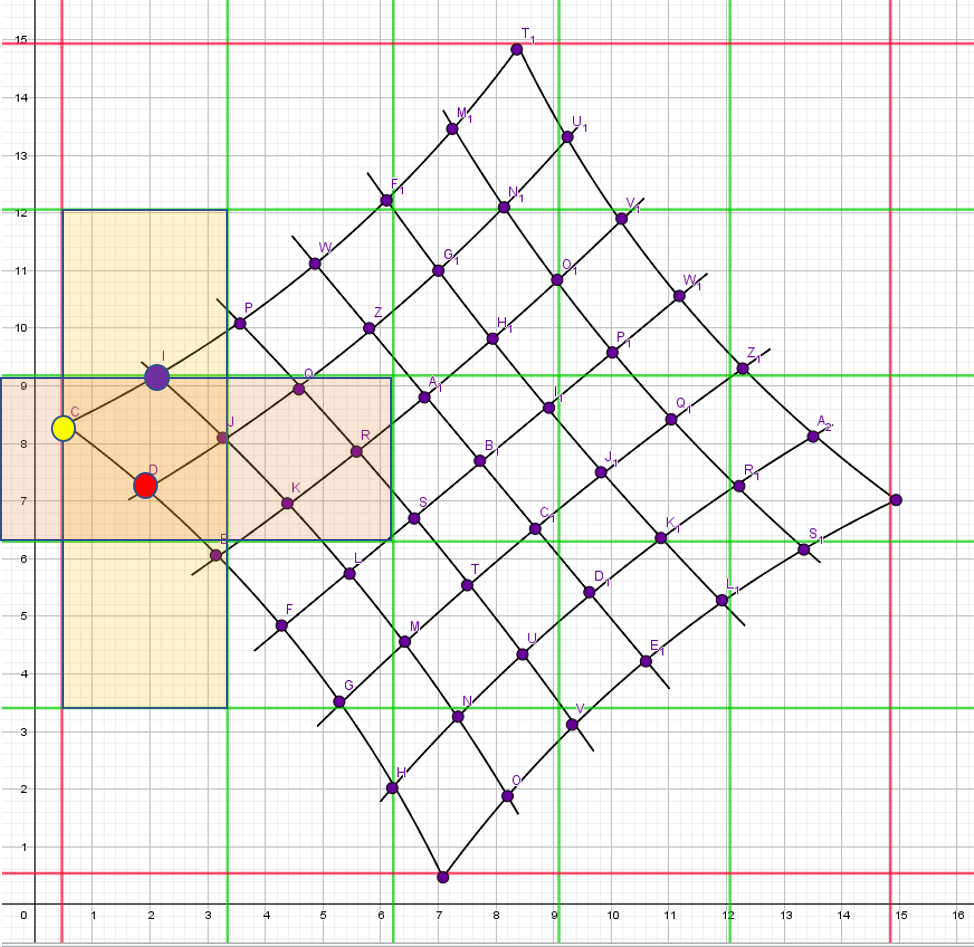
\includegraphics[width=0.6\linewidth]{images/VerzeichnetesSchachbrett_2.png}
	\caption[Finden der Startvektoren in Schachbrettpunkten]{Der in gelb markierte Bereich beinhaltet die für $NextI$ möglichen Punkte. der orange markierte Bereich beinhaltet die für $NextJ$ möglichen Punkte. Der violett gefärbe Punkt ist der gesuchte $NextI$, der rot gefärbte Punkt ist der gesuchte $NextJ$}
	\label{fig:NextINextJ}
\end{figure}


%Gibt es in diesem Bereich einen Punkt, dessen $y$-Koordinate größer ist als die $y$-Koordinate von $StartPoint$ und
%
%Gibt es in diesem Bereich einen Punkt, dessen $y$-Koordinate größer als die von $StartPoint$ ist 

Innerhalb des Bereichs wird der Punkt mit der zu $StartPoint$ nächst höheren $y$-Koordinate ermittelt. Dieser Punkt wird dann als vorläufiges $NextI$ festgelegt. Danach wird geprüft, ob das neu bestimmte $NextI$ bereits das letztendliche $NextI$ ist. Um das zu prüfen wird zunächst überprüft ob es innerhalb des gelben Bereichs noch einen Punkt gibt, dessen $x$-Koordinatenabstand vom Startpunkt aus kleiner gleich dem $x$-Koordinatenabstand zwischen dem momentanen $NextI$ zum Startpunkt ist. Gleichzeitig wird geprüft, ob der $y$-Koordinatenabstand zwischen $StartPoint$ und $NextI$ größer ist als der $y$-Koordinatenabstand zwischen einem anderen Punkt innerhalb des Suchbereichs und $StartPoint$. Ist dies der Fall, so wird der Punkt auf den beides zutrifft als neues $NextI$ bestimmt. In Abbildung \ref{fig:FindNextIJ} ist die Überprüfung on das erste $NextI$ bereits stimmt oder geändert werden muss nochmal grafisch veranschaulicht.\\

Die Suche nach dem nächsten Punkt in $j$-Richtung erfolgt nach dem gleichen Prinzip. Für $NextJ$ wird der in Abbildung \ref{fig:FindNextIJ} rot hinterlegte Bereich untersucht. Innerhalb des Roten Bereichs, wird derjenige Punkt ermittelt der zu $StartPoint$ den nächst höheren $x$-Wert besitzt. Dieser wird dann als vorläufiger $NextJ$ gespeichert. Danach wird auch über Abstandsrechnungen überprüft, ob es sich bei $NextJ$ bereits um den finalen Punkt handelt oder ob er nochmal geändert wird.\\

Die beiden Punkte $NextI$ und $NextJ$ werden dann wie $StartPoint$ um die zwei Schlüssel $NeighbourI$ und $NeighbourJ$ erweitert. Die Punkte sind dann wie folgt definiert und werden in die Liste $SortedPoints$ gespeichert. die auf die Koordinateninformation beschränkte Version der beiden Punkte, wird in die $CheckList$ gespeichert. Damit gelten $NextI$ und $NextJ$ als sortiert.


\begin{gather*}
	\begin{split}
		NextI &= \{ <|CoordI \rightarrow i-\text{Koordinate},\, CoordJ \rightarrow j-\text{Koordinat},\, \\
		&CellI \rightarrow i-\text{Zelle},\, CellJ \rightarrow j-\text{Zelle},\,
		NeighbourI \rightarrow 2, \,NeighbourJ \rightarrow 1  |>\}
	\end{split}\\
	\begin{split}
	NextJ &= \{ <|CoordI \rightarrow i-\text{Koordinate},\, CoordJ \rightarrow j-\text{Koordinat},\, \\
	&CellI \rightarrow i-\text{Zelle},\, CellJ \rightarrow j-\text{Zelle},\,
	NeighbourI \rightarrow 1, \,NeighbourJ \rightarrow 2 |>\}
\end{split}
\end{gather*}




\begin{figure}[!htb]
	\centering
	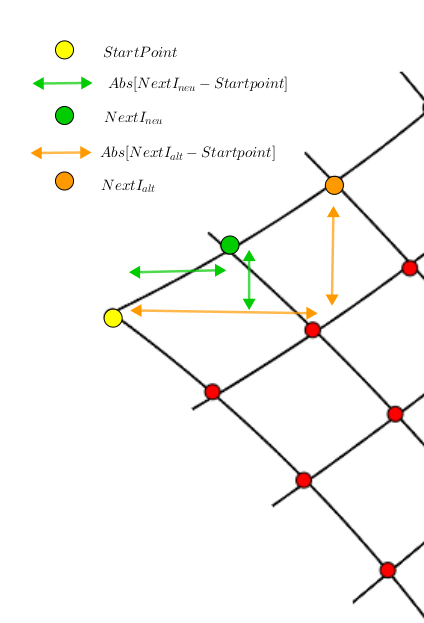
\includegraphics[width=0.5\linewidth]{images/SearchNextI.png}
	\caption[Überprüfung des gefundenen $NextI$]{Um zu überprüfen, ob der momentan $NextI$, in der Abbildung der orange Punkt, wirklich der nächste Punkt ist, wird sein Abstand zum Starpunkt in $j$- und  $i$- Richtung, mit den anderen noch möglichen Punkten verglichen. Gibt es einen dessen beide Abstände kleiner sind, wie beispielsweise der grüne Punkt, so wird dieser zum neuen $NextI$ bestimmt.}
	\label{fig:FindNextIJ}
\end{figure}
\pagebreak


Mit den Punkten $StartPoint$, $NextI$ und $NextJ$ können die ersten Richtungsvektoren in $i$-Richtung mit $NextIDir= NextI - StatPoint$ und $j$- Richtung mit $NextJDir =NextJ\,StatPoint$ gebildet werden. Anhand der Richtungsvektoren werden Suchbereiche definiert, in welchen der jeweils nächste Punkt in entsprechender Richtung $i$ oder $j$ gesucht werden soll.\\ 

% anhand welcher das Schachbrett Gitter rekonstruiert werden kann.

Für beide Richtungen wird die Anzahl der möglichen Punkte begrenzt. Es werden zwei Listen $IList$ und $JList$ angelegt. In $IList$ werden alle Punkte gespeichert welche die Zeleen Schlüssel $CellI_{min}$ bis $CellI_{max}$ und $CellJ_1$ und $CellJ_2$ gespeichert haben. In Abbildung \ref{fig:IListJList} entspricht das dem Vertikalen blauen Bereich. In $JList$, kommen alle Punkte deren Zellen Schlüssen $CellJ_{min}$ bis $CellJ_{max}$ und $CellI_1$ und $CellI_2$ gespeichert haben. Was dem horizontalen blauen Bereich in Abbildung \ref{fig:IListJList} entspricht. \\

Der Algorithmus dann nach folgendem Schema vor. Zu erst wird die Untere Schachbrettkante vervollständigt. Sprich alle Punkte de Später die Schlüssen $NeighbourI = 1$ und $NeighbourJ = j_{alle}$ haben sollen.\\

%Zuerst wird die erste Kante in $j$-Richtung

Neben dem Richtungsvekor $NextJDir$ wird noch ein Pufferwert $ProportionI$ deklariert, welcher den $i$-Koordinatenabstand zwischen $StartPoint$ und $NextJ$ beinhaltet. Dieser Pufferwert wird in positiver sowie in negativer Richtung um den Richtungsvektor definiert. In Abbildung \ref{fig:UebersichtSortierungsAlg} ist dieser Puffer als Blauer Kegel vor den Punkten zu sehen. Dieser Kegel definiert den Suchbereich von einem bereits bekannten Punkt zu einem noch unbekannten Punkt.

%
% 
% wird ein Richtungsvektor $NextJDir$ aus $StartPoint$ und $NextJ$ gebildet. Des Weiteren wird ein Pufferwert $ProportionI$ deklariert, welcher den $i$-Koordinatenabstand zwischen $StartPoint$ und $NextJ$ beinhaltet. Anhand des Richtungsvektors $NextJDir$ und des Pufferwertes $ProportionI$ wird der nächste Punkt von $NextJ$ aus gesucht. \\

\begin{gather*}
	NextJDir = NextI - StartPoint\\
	ProportionI = NextI[CoordI]-StartPoint[CoordI]
\end{gather*}\\

In Abbildung \ref{fig:IListJList} auf dem linken Bild wird der Richtungsvektor $NextJDir$ als Pfeil vom gelben $StartPoint$ zum roten $NextJ$ dargestellt, der Richtungsvektor wird noch um einen Pufferwert vergrößert. Die Pfeile welche in $i$-Richtung von $NextJ$ aus ausgehen, ist der Abstand $ProporionI$, welcher auf die $i$-Koordinate von $NextJ$ einmal addiert und einmal subtrahiert wird. Der Bereich den die Vektoren aufspannen bildet den Suchbereich für den auf $NextJ$ folgenden Punkt.\\


\begin{figure}[!htb]
	\centering
	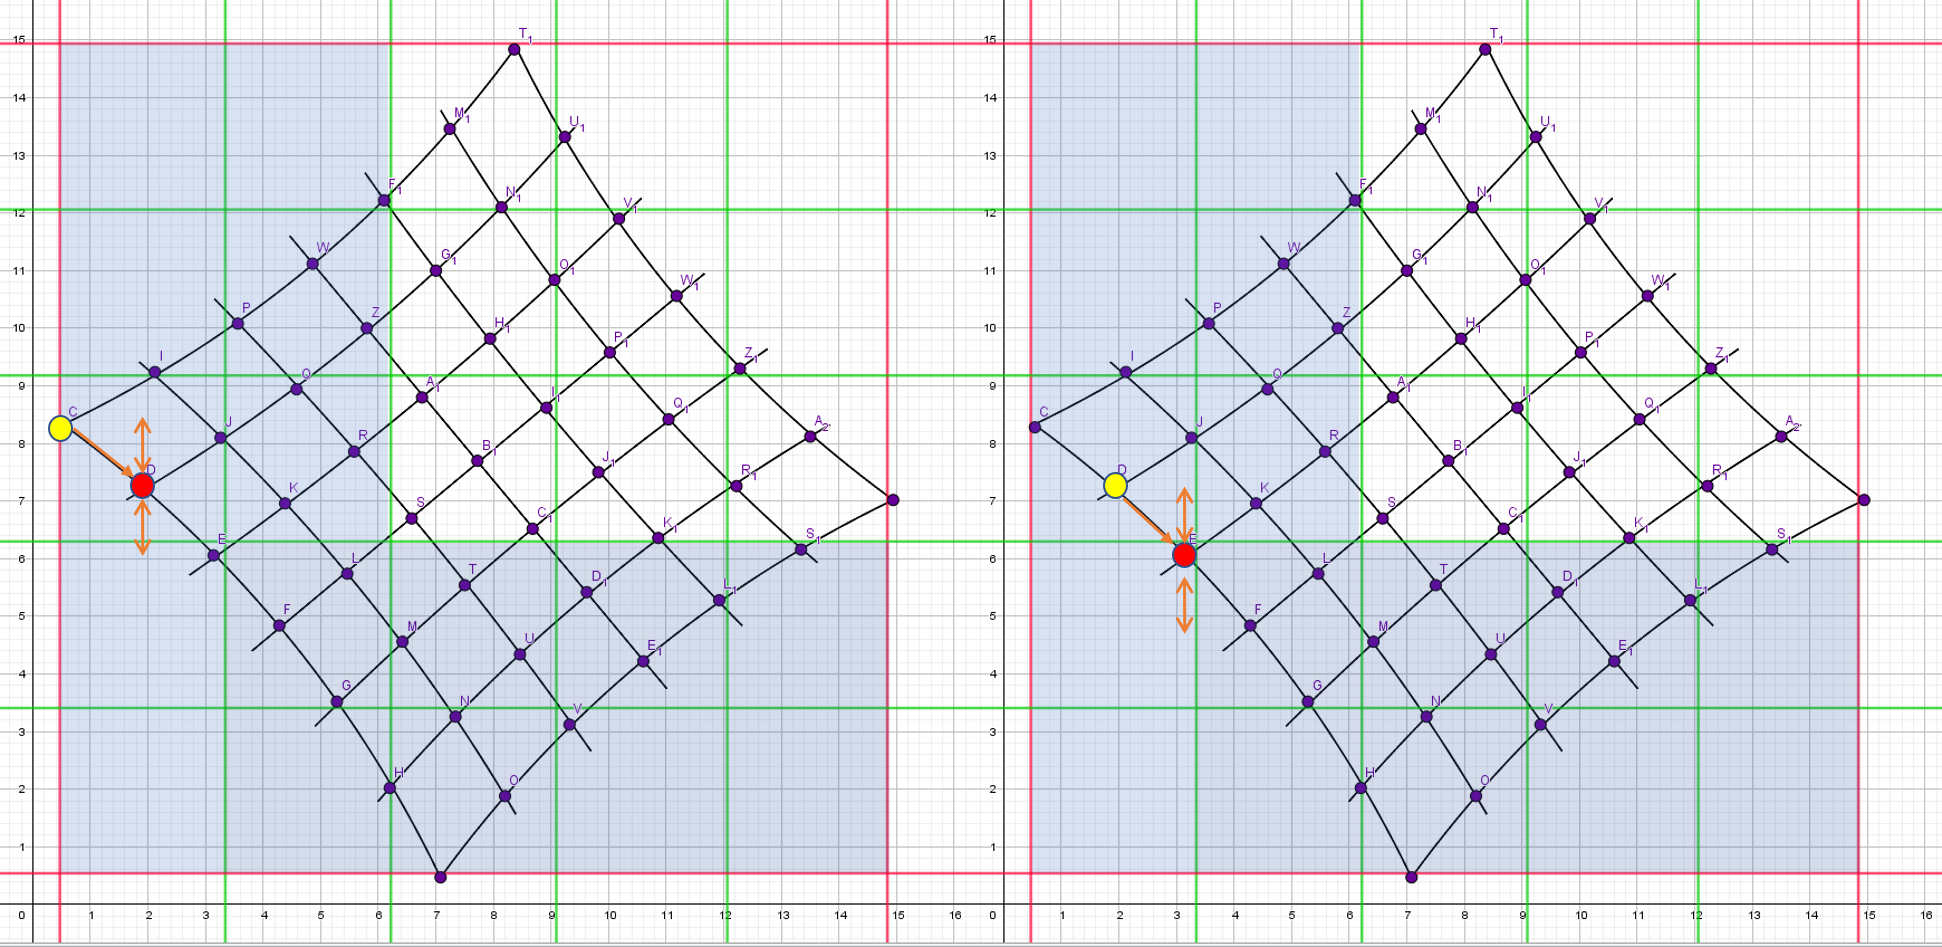
\includegraphics[width=0.8\linewidth]{images/VerzeichnetesSchachbrett_4.png}
	\caption[Suche nach $NextJ$]{Im linken Bild ist der Startpunkt in gelb dargestellt und der bereits gefundenen Punt $NextJ$ ist in rot eingefärbt. Anhand der beiden Punkte wird ein Richtungsvektor definiert und zwei Pufferwerte oberhalb und unterhalb. Diese bilden einen Suchbereich. Im rechten Bild wurde $NextJ$ als neuer Startwert festgelegt. Der zuvor definierte Suchbereich wird vor den neuen Startpunkt gesetzt und es wird nach einem potentiellen nächsten $NextJ$ gesucht.}
	\label{fig:IListJList}
\end{figure}

Für die weitere Such nach Punkten entlang der Kante wird in einer Schleife $NextJ$ zu neuen $StartPoint$. Der zuvor definierte Suchbereich wird vor den neuen $StatPoint$ definiert und nach einem neuen $NextJ$ gesucht. In Abbildung \ref{fig:FindNextIPoint} ist dieser Vorgang nochmal veranschaulicht. Wird ein Punkt in diesem Bereich entdeckt, so wird dieser zum neuen $NextJ$, sofern er sich noch nicht in der $CheckList$ befindet. Tritt der Fall ein, dass ein Punkt bereits in der $CheckList$ sich befindet, so wird dieser ignoriert. Der neu entdeckte Punkt wird zu $NextJ$. $NextJ $ wird dann wieder um die zwei Schlüssel $BeighbourI$ und $NeighbourJ$ erweitert und in die $SortedPoints$ Liste gespeichert und dessen verkürzte Fassung wird in die $CheckList$ geschrieben.\\

%Vom neuen $StartPoint$ ausgehend, wird der zuvor definierte Suchbereich nach einem neuem $NextJ$ abgesucht. 
%
%Die Position und der Platz im Schachbrettgitter werden dem neu entdeckten Punkt, wie die Punkten zuvor, durch Schlüsselwerte festgehalten und in die Liste $SortedList$ gespeichert. Des Weiteren wird auch dieser in die $CheckList$ aufgenommen.\\

Anhand des neuen $StartPoints$ und des neuen $NextJ$ werden der Richtungsvektor $NextJDir$ und $ProportionI$ neu berechnet. $NextJ$ wird wieder zum neuen $StartPoint$ und die Suche wird dementsprechend weiter geführt, bis kein Punkt mehr gefunden wird. Alle Punkte werden als $Asssociation$ mit der entsprechenden Erweiterung der Schlüsselwerte in $SortedList$ und $CheckList$ eingetragen.\\

Bevor die Suche entlang der beiden außen Kanten als beendet gilt, treten noch zwei Sicherheitsfunktionen in Kraft. Die erste wird als $Saftylist$ bezeichnet. Wird beispielsweise kein weiterer Punkt bei der Detektierung der außen Kanten innerhalb von $JList$ oder $IList$ gefunden, so wird der Suchbereich kurzfristig erweitert. Um den letzten gefundenen Punkt $NextJ$ oder auch $NextI$ werden, sofern vorhanden alle noch nicht abgesuchten Zellen um die Punkte herum abgesucht. Gibt es in einer darum liegenden Zelle noch einen Punkt, der in den Suchbereich fällt, wird dieser noch mit aufgenommen. Die Funktion der $SaftyList$ kommt beispielsweise genau dann zum Einsatz, wenn die Punkte eines Schachbretts wie in \ref{fig:SaftyList} sortiert werden. In der linken Abbildung ist zu sehen, dass der Brreich der $IList$ endet, es aber noch weitere Punkte gibt. Auf der rechten Abbildung ist dann zu sehen, wie der rot hinterlegte Bereich noch hinzugenommen wird und die restlichen Punkte auch noch gefunden werden.\\

%erweitert $Saftylist$ den Suchbereich um den letzten noch detektierten $NextJ$ um alle Zellen um diesen Punkt herum und überprüft, dann nochmal, ob es einen weiteren Punkt innerhalb des letzten definierten Suchbereiches gibt.
%
% Ist dies der Fall, so wird dieser Punkt auch noch mit aufgenommen. Ist dies nicht der Fall ist die Suche für die Reihe beendet. Die selbe Sicherheitsfunktion gibt es auch für die Suche in $i$-Richtung.\\
%
%In Abbildung \ref{fig:SaftyList} auf dem rechten Bild ist ein Beispiel für den Einsatz der $SaftyList$-Funktion zu sehen. Der rote Bereich vom gelben Punkt aus gehend ist definiert als der Bereich potentieller weiterer Punkte außerhalb der $IList$.\\

Ist die unterste Kante in $j$-Richtung bestimmt, so wird die nächste Reihe vervollständigt, beginnend am Punkt $NextI$. $NextI$ ist der neue $StartPoint$ von wo aus die nächste Reihe in $j$-Richtung vervollständigt wird. Bevor die nächste Reihe vervollstädnigt werden kann, muss zuerset der nächste Punkt $NextI$ auf der äußeren Kante bestimmt werden. Wie in den Abbildung \ref{fig:FindNextIPoint} und \ref{fig:SaftyList} zu sehen, basiert die Suche nach $NextI$ auf dem gleichen Verfahren wie die Suche nach $NextJ$.\\


\begin{figure}[!htb]
	\centering
	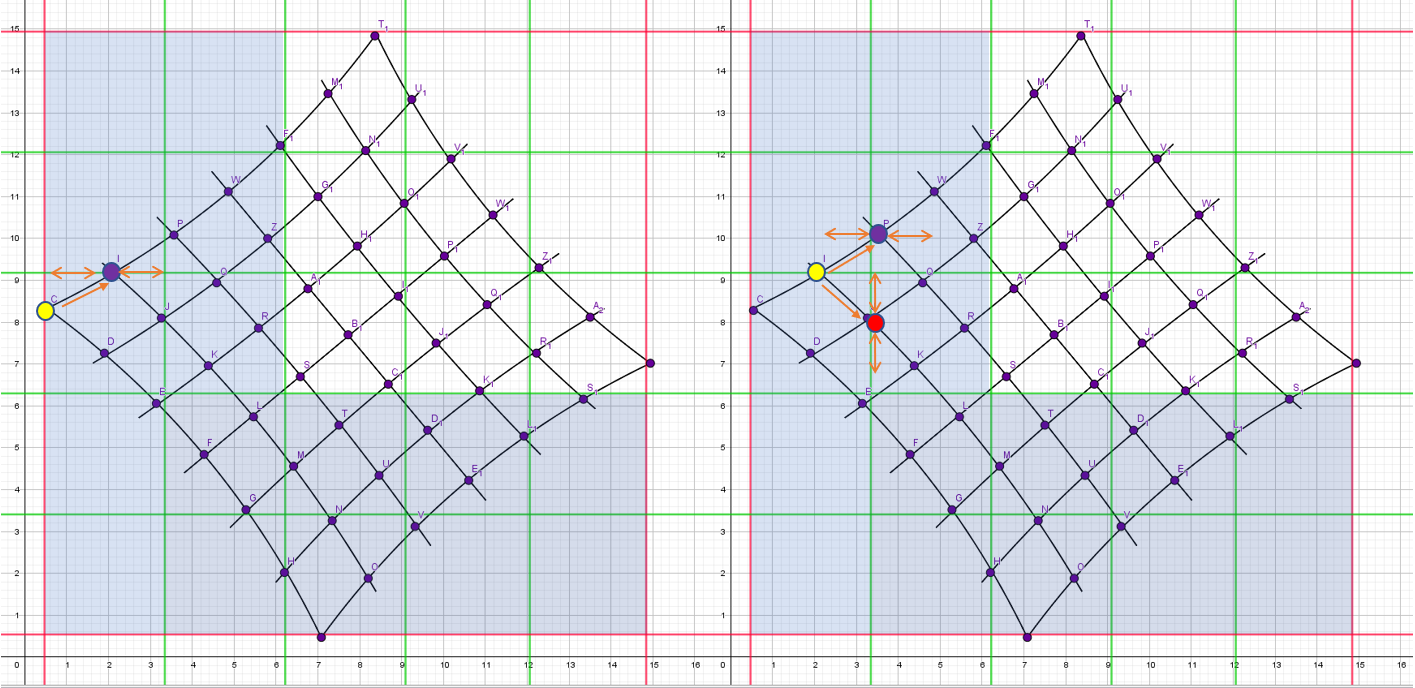
\includegraphics[width=0.8\linewidth]{images/VerzeichnetesSchachbrett_5.png}
	\caption[Suche nach dem nächsten $NextI$]{Die Suche nach dem nächsten $NextI$ basiert auf dem selben Verfahren wie die Suche nach $NextJ$. Sobald ein neuer $NextI$ gefunden wurde, wird die Reihe in $j$-Richtung vervollständigt, bevor es mit dem nächsten $NextI$ weiter geht}
	\label{fig:FindNextIPoint}
\end{figure}

\begin{figure}[!htb]
	\centering
	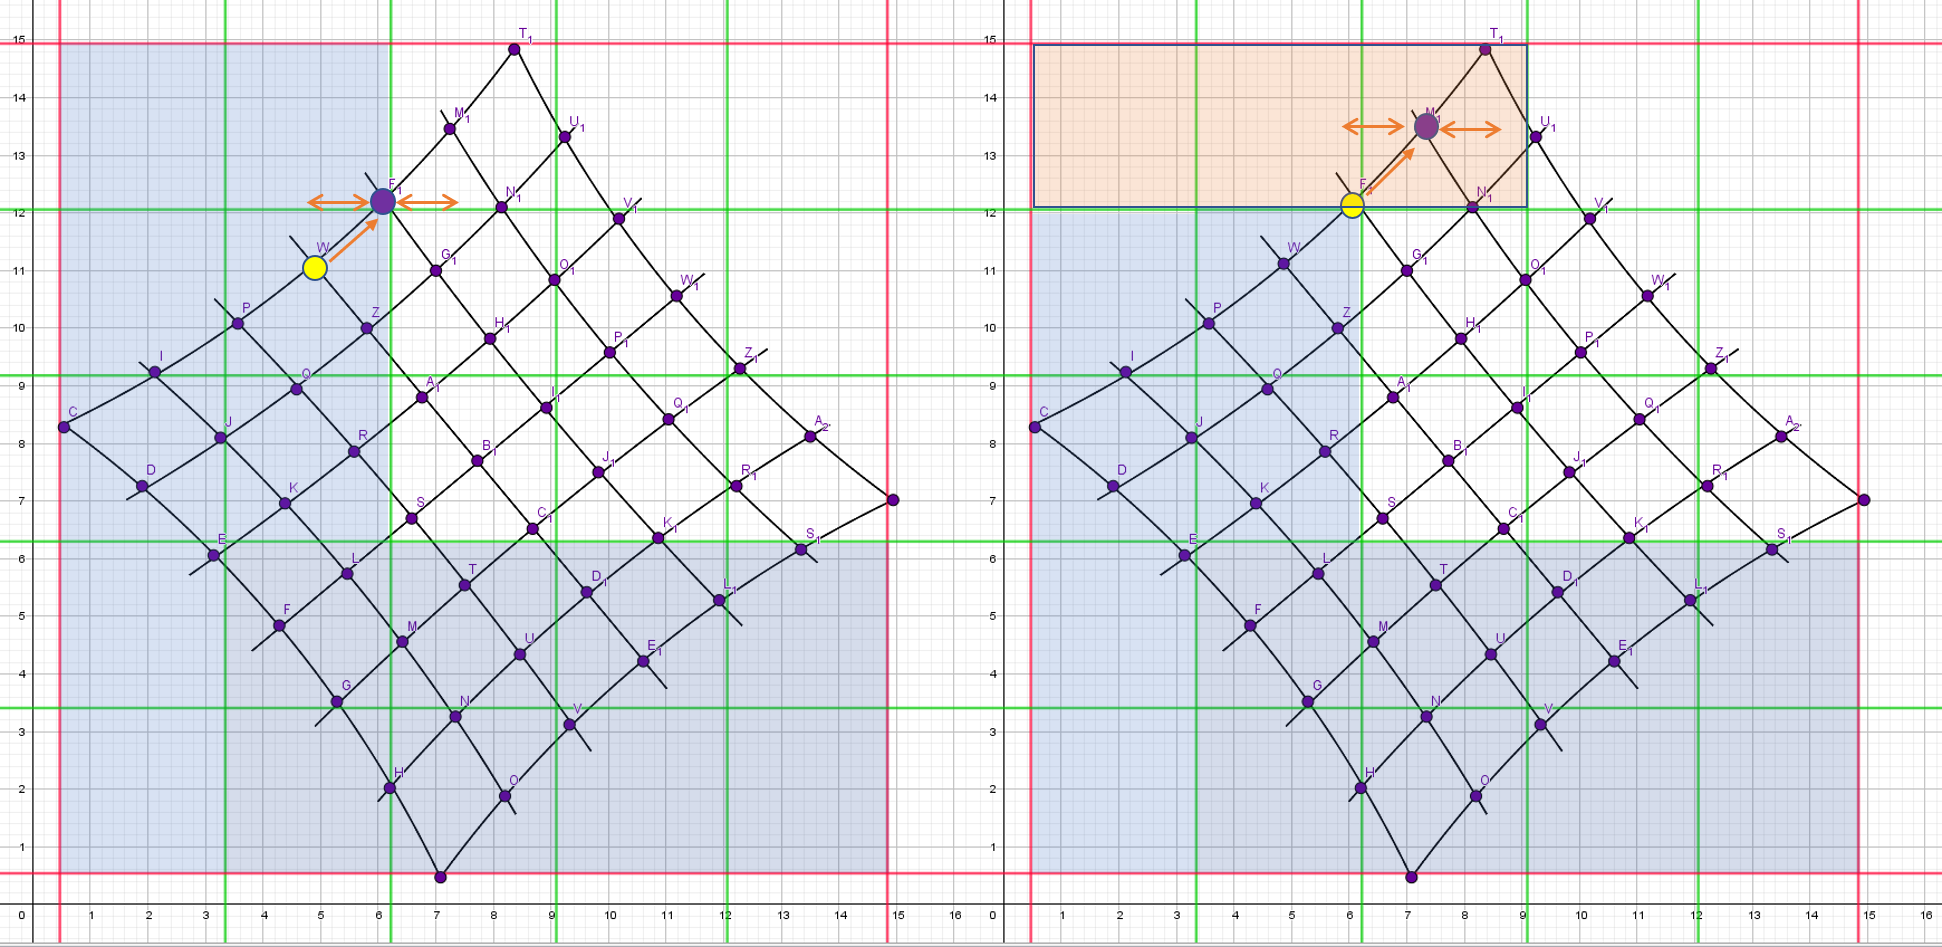
\includegraphics[width=0.8\linewidth]{images/VerzeichnetesSchachbrett_6.png}
	\caption[Sicherheitsfunktion $SaftyList$]{Wird der kein weiterer Punkt innerhalb von $IList$ oder $JList$ gefunden, Wird ein kleiner Bereich, hier in rot hinterlegt, abgesucht, ob es doch noch potentielle nächste Punkte gibt, die aufgrund der Lage des Schachbretts nich in $IList$ oder $JList$ mit enthalten waren}
	\label{fig:SaftyList}
\end{figure}


Zuvor wurde erwähnt, dass es neben $SaftyList$ noch eine andere Sicherheitsfunktion namens gibt. Hierzu sei nochmal erwähnt, dass der hier beschriebene Sortierungsalgorithmus auf einem bereits bestehenden Algorithmus aufbaut. Dieser Algorithmus detektiert Die Eckpunkte eines Schachbretts und speichert die Bildkoordinaten in eine Liste. Bei der Detektion kann es vorkommen, dass Punkte, durch beispielsweise Rauschen oder Bildunschärfen, nicht erkannt werden und somit Lücken im Schachbrettgitter entstehen. Ist dies der Fall würde der Sortierungsalgorithmus wie er bis jetzt ist, bei einer Lücke mit der Suche aufhören, da kein Punkt im definierten Suchbereich gefunden werden kann. Weitere Punkte welche sich je nach dem hinter der Lücke befinden, würde so nicht mehr gefunden und sortiert werden können. Diese Punkte würde nicht in der Liste $SortedList$ landen und der Algorithmus würde dich Nachricht ausgeben, dass die Sortierung unvollständig sei.\\

Um dem entgegen zu wirken wurde die Sicherheitsfunktion $PlaceSyntheticPoint$ entwickelt. Sollte vorerst kein Punkt im Suchbereich entdeckt, werden, so setzt die Sicherheitsfunktion einen synthetischen Punkt und sucht ausgehend von diesem synthetischen weiter nach Punkten. Sollte ein Punkt nach dem synthetischen Punkt gefunden werden, so bleibt der synthetische Punkt bestehen und die Suche wird normal fortgesetzt. Der synthetische Punkt wird nicht in die Liste $SortedList$ mit aufgenommen, da er später nicht als möglicher korrespondierender Punkt in betrachtet gezogen werden soll. Er dient lediglich dazu alle real vorhandenen Punkte zu finden und richtig zu sortieren.
Wird nach dem setzten des synthetischen Punkt kein weiterer Punkt gefunden, gilt die Suche in der Reihe beziehungsweise Spalte für beendet und der synthetische Punkt wieder wieder gelöscht. \\


% die Nachricht ausgeben, dass die Sortierung der
%
%Ist dies der Fall entstehen Lücken im Schachbrettmuster und der Sortierungsalgorithmus, würde nicht alle Punkte richtig sortieren könne.\\
%
%
%Entspricht die Anzahl der Listeneinträge in $SortedPoints$ der Anzahl der vom Algorithmus entgegengenommenen Anzahl, sind alle Punkte sortiert worden.


In Abbildung \ref{fig:ChessBoardLeft} und \ref{fig:ChessBoardRight} wird ein Schachbrett aus zwei unterschiedlichen Blickwinkeln dargestellt. Die roten Punkte markieren die Eckpunkte, deren Koordinaten an den Sortierungsalgorithmus übergeben werden. In den Abbildungen \ref{fig:ChessBoardLeftAlg} und \ref{fig:ChessBoardRightAlg} werden alle Punkte, welche in der Liste $SortedPoints$ gespeichert wurden in einem Plot ausgegeben. Es wird gesagt, dass alle Punkte deren Schlüssel $NeighbourI = 3$ ist, in grün dargestellt werden sollen. Das Ergebnis dieser Abfrage ist ebenfalls in den Abbildungen \ref{fig:ChessBoardLeftAlg} und \ref{fig:ChessBoardRightAlg} zu sehen. Der entstandene Sortierungalgorithmus ist also in der Lage aus Bildern zweier Schachbretter gleiche Eckpunkte und somit korrespondierende Punkte zu detektieren. Soll ein einzelner Punkt Abgefragt wollen, so für die Schlüssel $NeighbourI$ und $NeighbourJ$ jeweils ein Wert abgefragt werden.


\begin{figure}[!htb]
	\minipage{0.47\textwidth}
	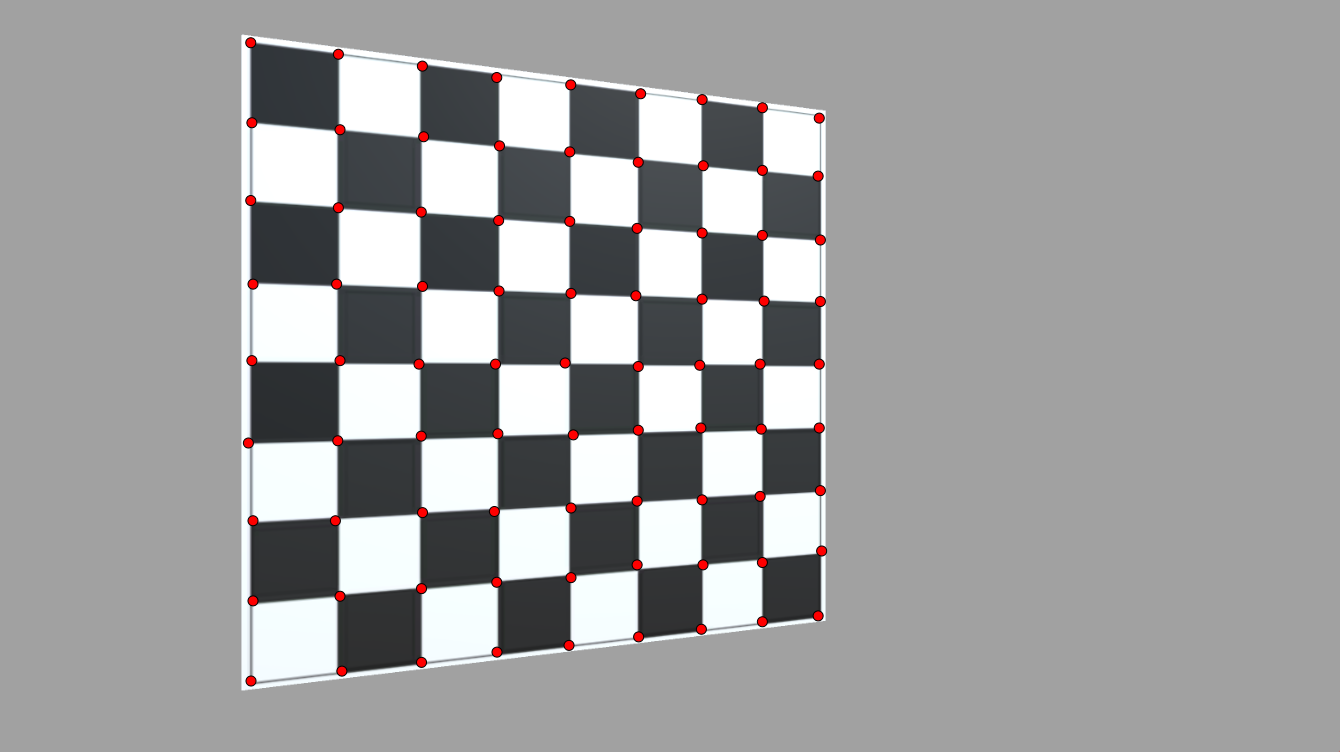
\includegraphics[width=\linewidth]{images/ChessBoardLeft.png}
	\caption[Korrespondezsuche mit Sortierungsalgorithmus. Schachbrett auf linker Seite]{Die Kamera,welche das Schachbrett abbildet steht links versetzt zum Schachbrett und ist rotiert}
	\label{fig:ChessBoardLeft}
	\endminipage\hfill
	\minipage{0.48\textwidth}
	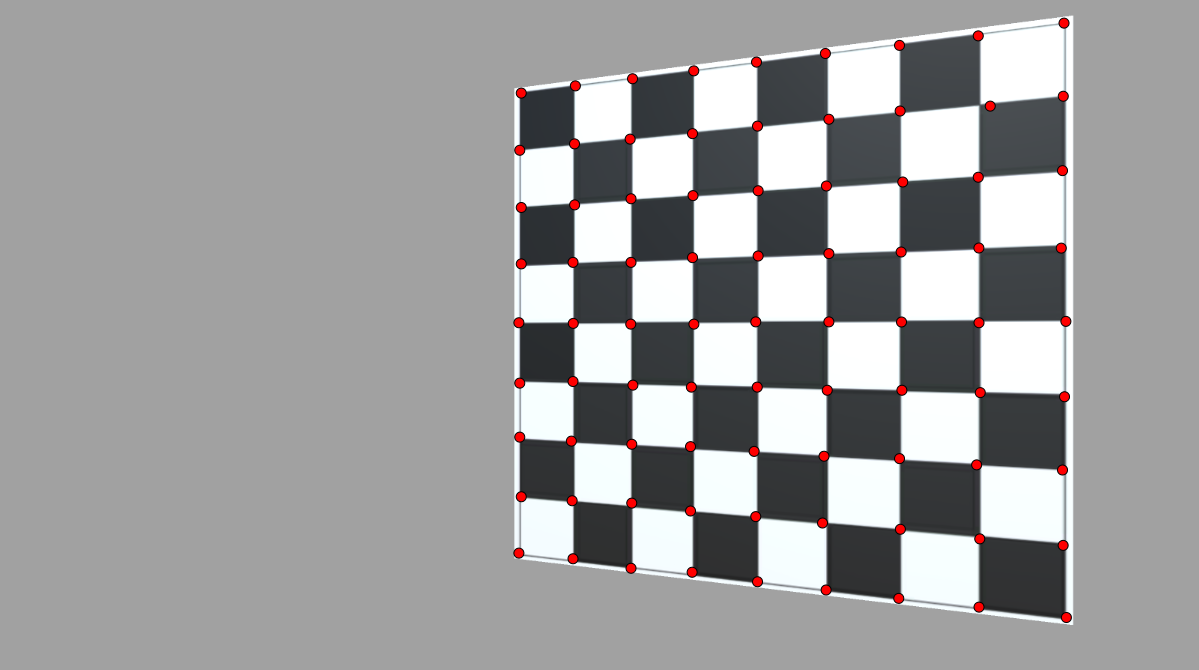
\includegraphics[width=\linewidth]{images/ChessBoardRight.png}
	\caption[Korrespondezsuche mit Sortierungsalgorithmus. Schachbrett auf rechter Seite]{Die Kamera, welche das Schachbrett abbildet steht rechts versetzt zum Schachbrett und ist rotiert}
	\label{fig:ChessBoardRight}
	\endminipage\hfill
\end{figure}


\begin{figure}[!htb]
	\minipage{0.48\textwidth}
	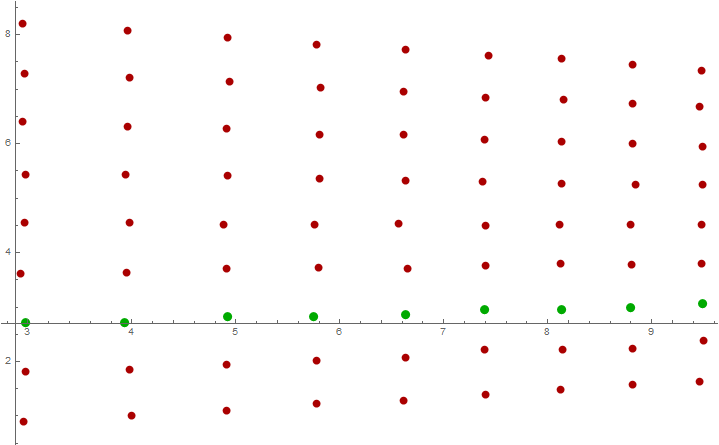
\includegraphics[width=\linewidth]{images/ChessBoardLeftAlg.png}
	\caption[Ergebnis des Sortierungsalgorithmus. Schachbrett auf linker Seite]{Die Abbidlung zeigt das Ergebnis der Sortierung des linken Schachbretts. In grün ist die Reihe an Punkten zu sehen, welche den Schlüssel $NeighbourI = 3$ haben.}
	\label{fig:ChessBoardLeftAlg}
	\endminipage\hfill
	\minipage{0.48\textwidth}
	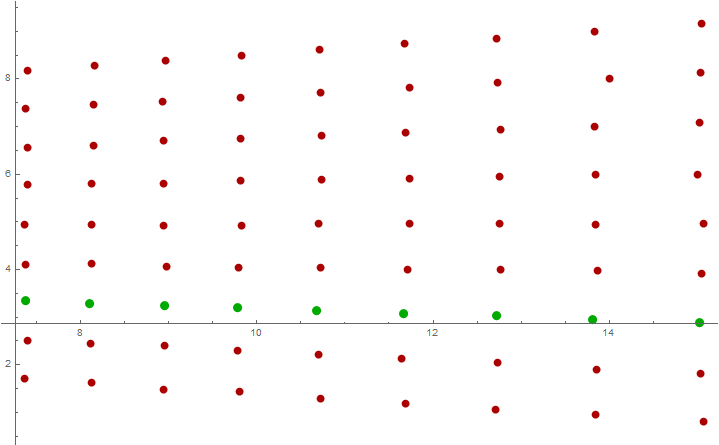
\includegraphics[width=\linewidth]{images/ChessBoardRightAlg.png}
	\caption[Ergebnis des Sortierungsalgorithmus. Schachbrett auf linker Seite]{Die Abbidlung zeigt das Ergebnis der Sortierung des rechten Schachbretts. In grün ist die Reihe an Punkten zu sehen, welche den Schlüssel $NeighbourI = 3$ haben.}
	\label{fig:ChessBoardRightAlg}
	\endminipage\hfill
\end{figure}
\pagebreak


\section{Resultate bei stark verzerrten Schachbrettern}
\label{sec:SchachAlgBeispiele}


Der entstandenen Sortierungsalgorithmus wird an stark perspektivisch Verzerrten oder durch Bildfehler wie Verzeichnungen betroffenen Schachbrettern getestet. Die Möglichkeit herauszufinden, welche Eckpunkte in einem stark verzerrten Bild eines Schachbretts in eine Reihe oder Spalte gehören, kann bei der mathematischen Entzerrung der Bilder von Nutzen sein. Dieser Vorteil war mit ein Grund warum der Algorithmus auf Grundlage von stark verzerrten Schachbrettbilder entwickelt wurde.\\

In den folgenden Beispielen sieht man jeweils das Originalbild des Schachbretts und neben dran die Ausgabe des Algorithmus. Der Plot zeigt alle Punkte an, welche in $SortedPoints$ aufgenommen wurden. Alle Punkte, welche als Schlüssel $NeighbourI = 3$ haben, wurden im folgenden grün eingefärbt, die restlichen Punkte sind rot gefärbt.


\begin{figure}[!htb]
	\minipage{0.48\textwidth}
	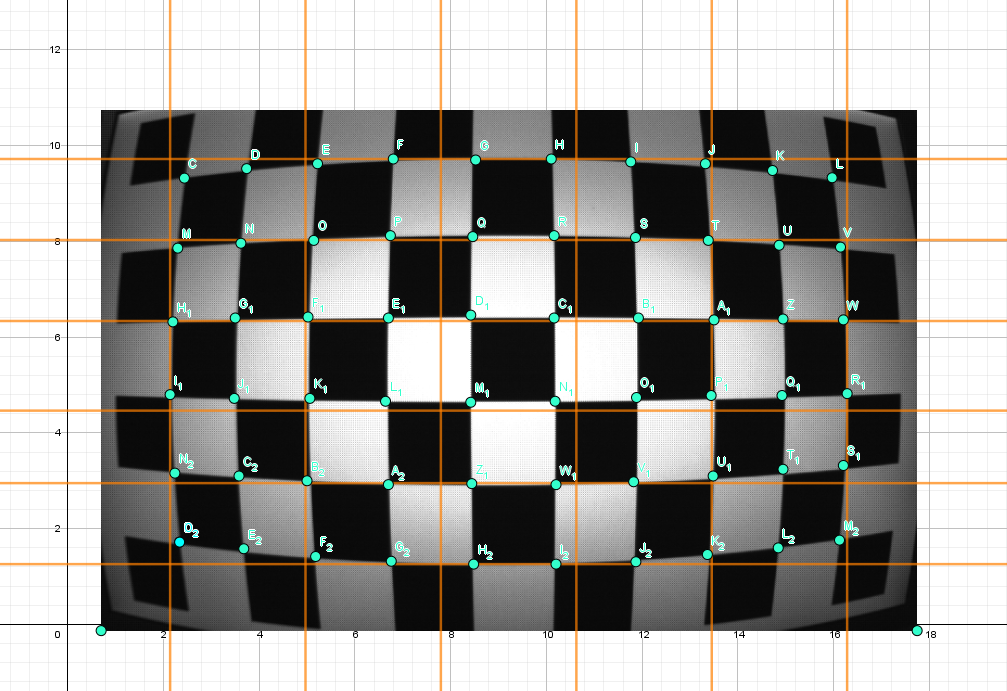
\includegraphics[width=\linewidth]{images/Tonnenverzeichnung.png}
	\caption[Schachbrett mit Tonnenverzeichnung]{Schachbrett mit Tonnenverzeichnung}
	\label{fig:Extreme1}
	\endminipage\hfill
	\minipage{0.48\textwidth}
	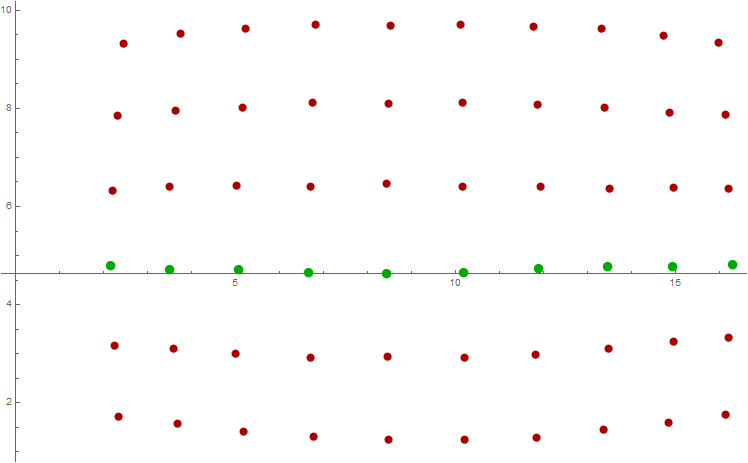
\includegraphics[width=\linewidth]{images/AlgTonnenverzeichnung.png}
	\caption[Sortierte Punkte eines Schachbretts mit Tonnenverzeichnung]{Ergebnis des Sortierungsalgorithmus.}
	\label{fig:Extreme2}
	\endminipage\hfill
\end{figure}

\begin{figure}[!htb]
	\minipage{0.45\textwidth}
	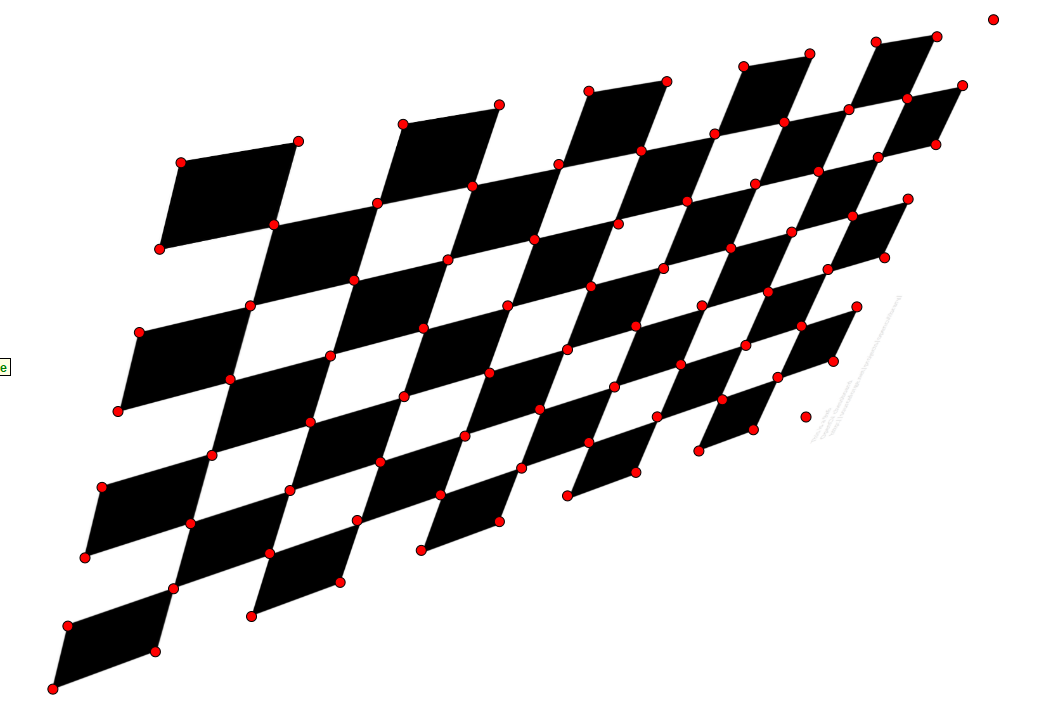
\includegraphics[width=\linewidth]{images/perspektivisch.png}
	\caption[perspektivisch startk verzerrtes Schachbrett]{Perspektivisch stark verzerrtes Schachbrett}
	\label{fig:Extreme3}
	\endminipage\hfill
	\minipage{0.49\textwidth}
	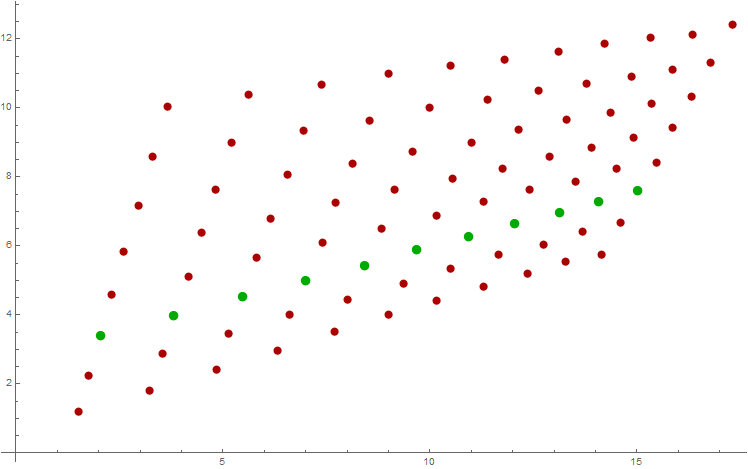
\includegraphics[width=\linewidth]{images/AlgPerspektifisch.png}
	\caption[Sortierte Punkte eines perspektivisch verzerrten Schachbretts]{Ergebnis des Sortierungsalgorithmus.}
	\label{fig:Extreme4}
	\endminipage\hfill
\end{figure}


\begin{figure}[!htb]
	\minipage{0.48\textwidth}
	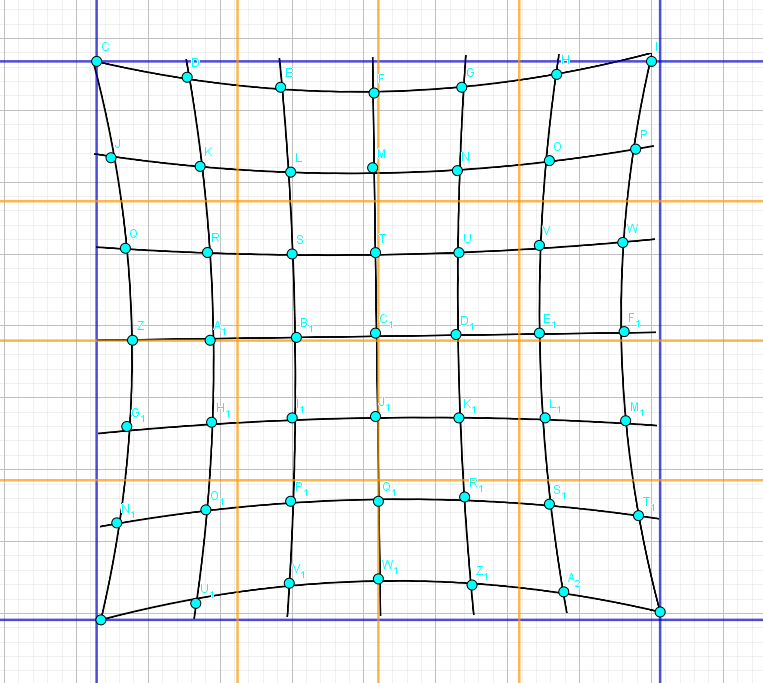
\includegraphics[width=\linewidth]{images/KissenVerzeichnung.png}
	\caption[Schachbrett mit Kissenverzeichnung]{Schachbrett mit Kissenverzeichnung}
	\label{fig:Extreme5}
	\endminipage\hfill
	\minipage{0.50\textwidth}
	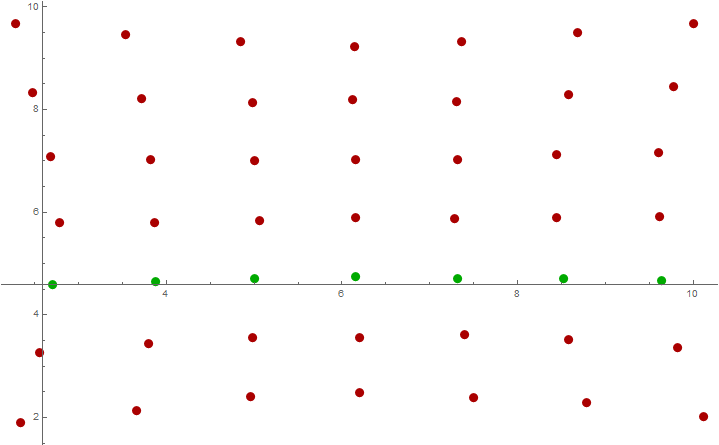
\includegraphics[width=\linewidth]{images/AlgKissen.png}
	\caption[Sortierte Punkte eines Schachbretts mit Kissenverzeichnung ]{Ergebnis des Sortierungsalgorithmus.}
	\label{fig:Extreme6}
	\endminipage\hfill
\end{figure}

\begin{figure}[!htb]
	\minipage{0.48\textwidth}
	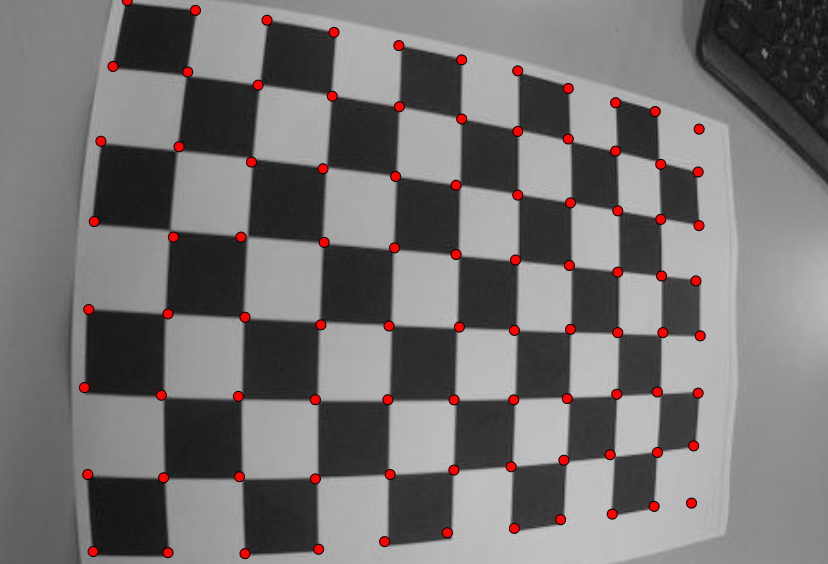
\includegraphics[width=\linewidth]{images/Tonnenverzeichnung_Perspektivisch.png}
	\caption[Perspektivisch verzerrtes Schachbrett mit Tonnenverzeichnung]{Perspektivisch verzerrten Schachbrett mit Tonnenverzeichnung}
	\label{fig:Extreme7}
	\endminipage\hfill
	\minipage{0.48\textwidth}
	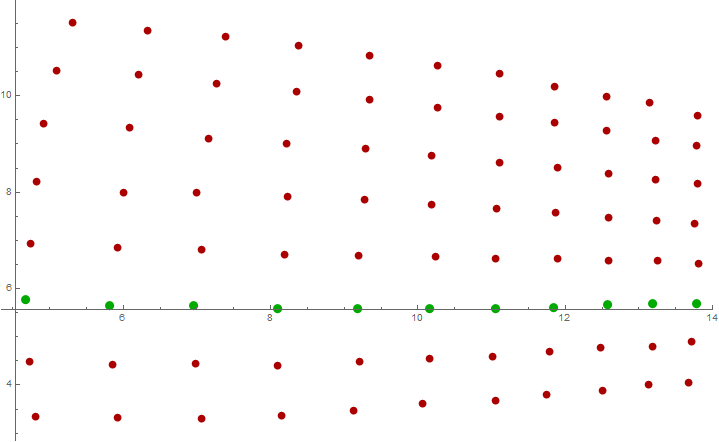
\includegraphics[width=\linewidth]{images/Tonnenverzeichnung_Perspektivisch_Alg.png}
	\caption[Sortieret Punkte eines perspektivisch verzerrten Schachbretts mit Tonnenverzeichnung]{Ergebnis des Sortierungsalgorithmus.}
	\label{fig:Extreme8}
	\endminipage\hfill
\end{figure}

\begin{figure}[!htb]
	\minipage{0.48\textwidth}
	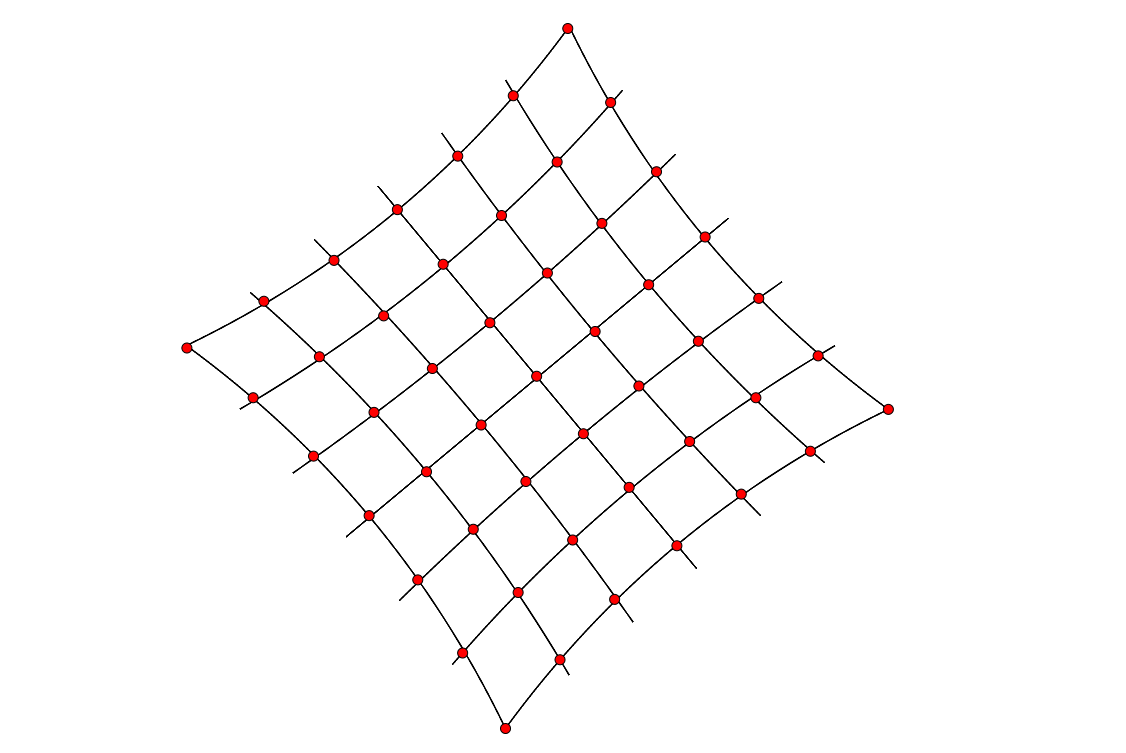
\includegraphics[width=\linewidth]{images/extrBsp.png}
	\caption{Bild eines Tonnenförmig verzeichnetem leicht perspektivisch verzerrtem Schachbretts}
	\label{fig:Extreme9}
	\endminipage\hfill
	\minipage{0.48\textwidth}
	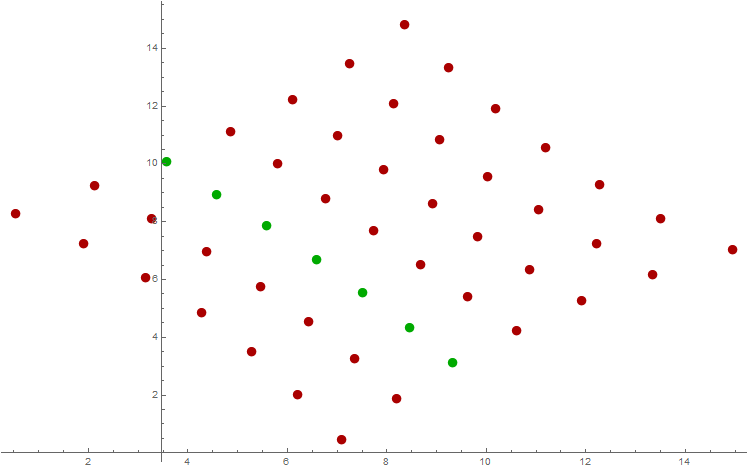
\includegraphics[width=\linewidth]{images/AlgExtrBsp.png}
	\caption{Algorithmisch detektierte Linie der dritten i-Reihe}
	\label{fig:Extreme10}
	\endminipage\hfill
\end{figure}


%\section{Modulübersicht}
%
%
%\begin{minipage}{\linewidth}
%	\centering
%	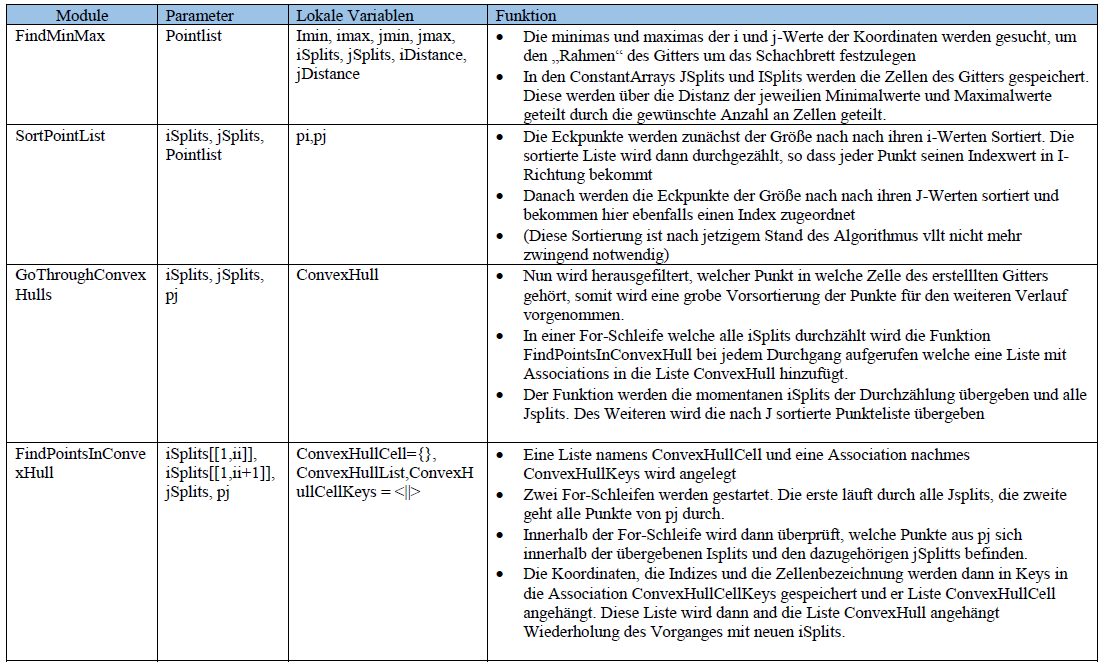
\includegraphics[width=1\linewidth]{images/KD1.png}
%	\captionof{figure}{Klassendiagramm}
%\end{minipage}
%\begin{minipage}{\linewidth}
%	\centering
%	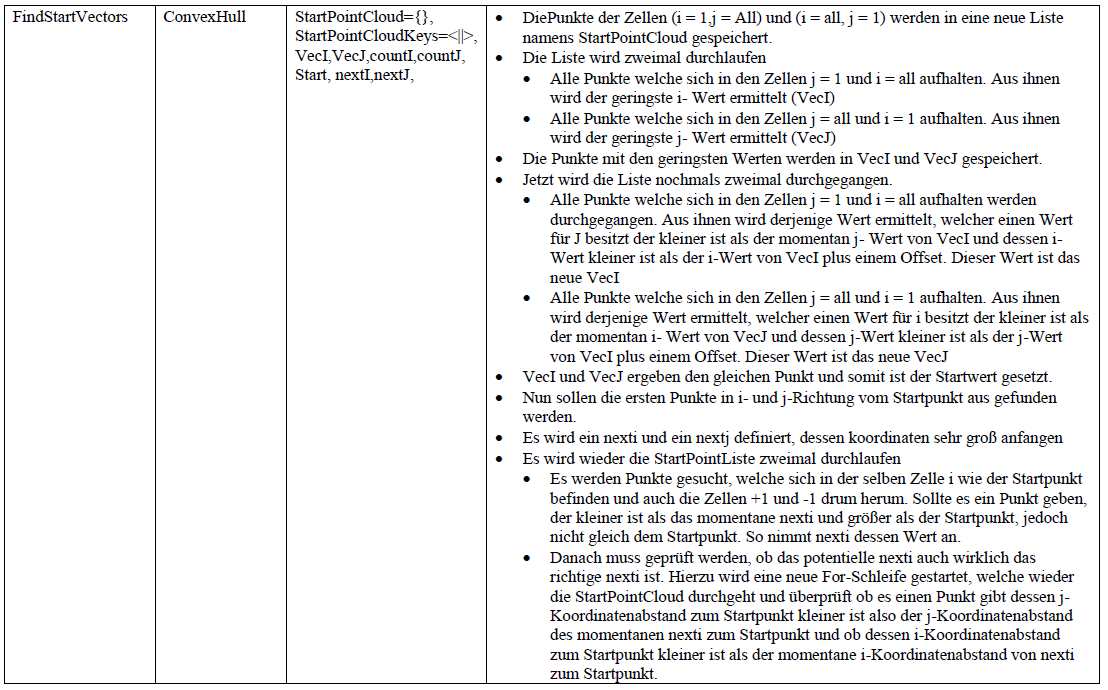
\includegraphics[width=1\linewidth]{images/KD2.png}
%	\captionof{figure}{Klassendiagramm}
%\end{minipage}
%\begin{minipage}{\linewidth}
%	\centering
%	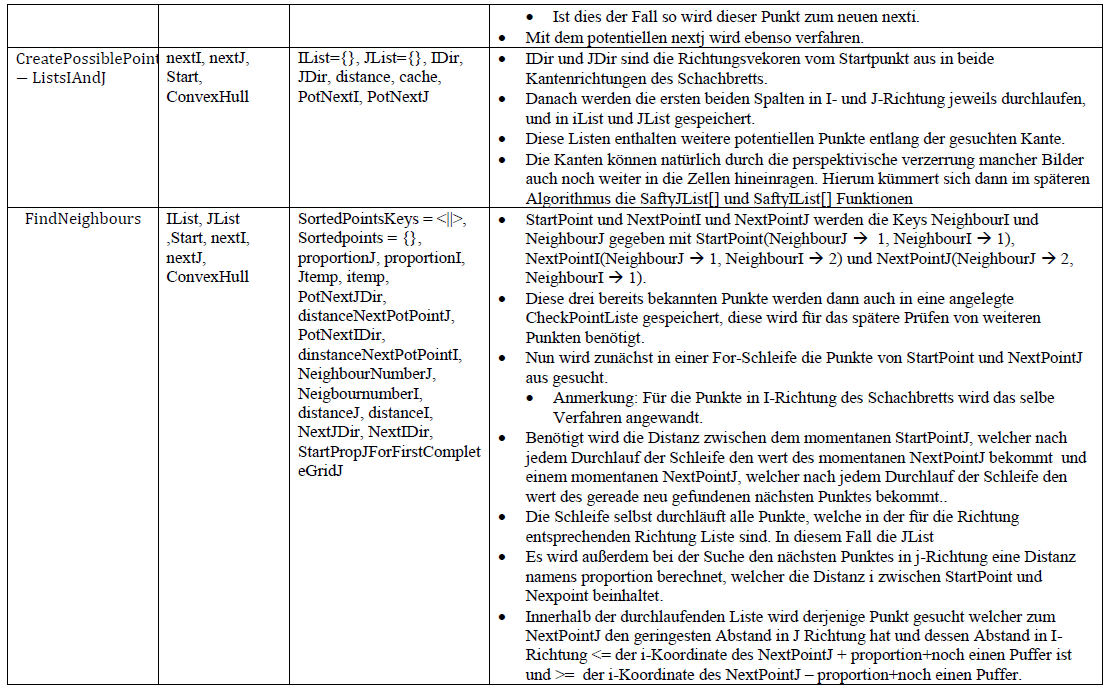
\includegraphics[width=1\linewidth]{images/KD3.png}
%	\captionof{figure}{Klassendiagramm}
%\end{minipage}
%\begin{minipage}{\linewidth}
%	\centering
%	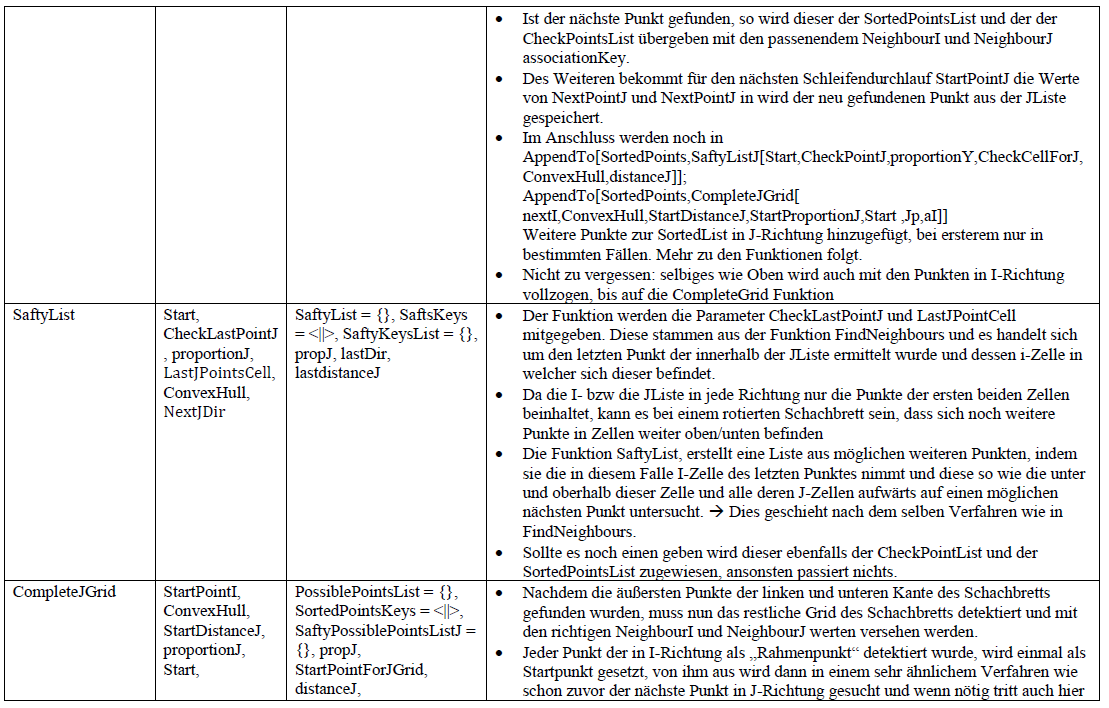
\includegraphics[width=1\linewidth]{images/KD4.png}
%	\captionof{figure}{Klassendiagramm}
%\end{minipage}
%\begin{minipage}{\linewidth}
%	\centering
%	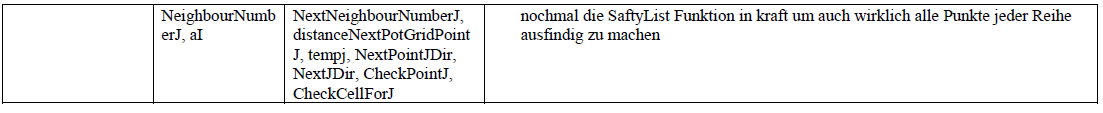
\includegraphics[width=1\linewidth]{images/KD5.png}
%	\captionof{figure}{Klassendiagramm}
%\end{minipage}\\


%Modulübersicht vllt in den Anhang??






